%%% Clinic Statement of Work Template
%%%
%%% C.M. Connelly <cmc@math.hmc.edu>
%%%
%%%  $Id: statement-of-work-template.tex 353 2010-08-23 23:47:44Z cmc $


%%% !!! HMC STUDENTS SHOULD REMOVE THE FOLLOWING COPYRIGHT NOTICE FROM
%%% !!! FINAL SUBMISSIONS.

%%% Copyright (C) 2004-2010 Department of Mathematics, Harvey Mudd College.
%%%
%%% This file is part of the hmcclinic class document provided to
%%% HMC mathematics students.
%%%
%%% See the COPYING document, which should accompany this
%%% distribution, for information about distribution and
%%% modification of the document and its components.

%%% !!! END COPYRIGHT NOTICE.


%%% Clinic reports use the clinic class, which should be located
%%% somewhere in TeX's search path.

%%% For your ``statement of work'' (or ``work statement''), specify
%%% the ``proposal'' document-class option to the hmcclinic class.
\documentclass{hmcclinic}
\usepackage{graphicx}
\usepackage{enumerate}
\usepackage{paralist}

%%% The major difference between the statement of work and a midyear
%%% or final report is that the statement of work is typeset as an
%%% article, which means that the highest level of structural
%%% division available to you is section rather than chapter.

%%% There are also some changes in pagination styles and content
%%% that reflect the briefer nature of the proposal.  For example,
%%% in the longer reports, you use \frontmatter, \mainmatter, and
%%% \backmatter to separate some sections of the report from
%%% others.  In the statement of work, you don't need those
%%% commands, as no such division is necessary.

%%% Other packages needed by your document may be loaded here.
% \usepackage{url}              % For formatting URLs and other web or
                                % file references.

%%% Provide additional context around errors. 
\setcounter{errorcontextlines}{1000}


%%% Information about this document.

%%% I find it most useful to put identifying information about a
%%% document near the top of the preamble.  Technically, this
%%% information must precede the \maketitle command, which often
%%% appears immediately after the beginning of the document 
%%% environment.  Placing it near the top of the document makes it
%%% easier to identify the document, and keeps it out from getting
%%% mixed up with the real meat of the document.

%%% We use the same set of commands for specifying information about
%%% the people involved with the project that are used in the longer
%%% reports, so you can copy most of this information directly into
%%% your midyear and final reports.

%%% So, some questions.

%% What is the name of the company or organization sponsoring your project?
\sponsor{SpaceX}

%% What is the title of your report?
\title{Process Time Analysis In Spaceflight}

%% Who are the authors of the report (your team members)?  (Separate
%% names with \and.)
\author{Wendy Brooks~(Fall Project Manager) \and May Lynn Forssen~(Spring Project Manager) \and Alix Joe \and
Rachel Macfarlane}

%% What is your faculty advisor's name?  (Again, separate names with
%% \and, if necessary.)
\advisor{Ben Wiedermann}

%% Liaison's name or names?
\liaison{Jim Gruen \and Jessica Hester '13 \and Jesse Keller }

%%% End of information section.

%%% New commands and environments.

%%% You can define your own commands and environments here.  If you
%%% have a lot of material here, you might want to consider splitting
%%% the commands and environments into a separate ``style'' file that
%%% you load with \usepackage.

\newcommand{\coolcommand}[1]{#1 is cool.} % Lets everyone know that
                                % the person or thing that you provide
                                % as the argument to the command is
                                % cool.

\newcommand{\tracecmd}{\fontfamily{pcr}\selectfont trace-cmd}

%%% Some theorem-like command definitions.

%%% The \newtheorem command comes from the amsthm package.  That
%%% package is loaded by the class file.

%%% Note that these definitions have changed from the version in the
%%% sample report document by dropping the ``within'' argument.  See
%%% Gratzer's _Math into LaTeX_ or the AMS-LaTeX documentation for
%%% more details.

% \newtheorem{thm}{Theorem}
% \newtheorem{Theo1}{Theorem}
% \newtheorem{Theo2}{Theorem}
% \newtheorem{Lemma}{Lemma}


%%% If you find that some words in your document are being hyphenated
%%% incorrectly, you can specify the correct hyphenation using the
%%% \hyphenation command.  Note that words are separated by
%%% whitespace, as shown below.

\hyphenation{ap-pen-dix wer-ther-i-an}


%%% The start of the document!

%% The document environment is the main environment in any LaTeX
%% document.  It contains other environments, as well as your text.

\usepackage{float}
\restylefloat{table}
\begin{document}

%%% In a longer document (such as your midterm and final reports),
%%% you would have separate \frontmatter, \mainmatter, and
%%% \backmatter commands to define some large chunks of your
%%% document.  For the Statement of Work, which is a short document,
%%% we don't need these commands.

%%% Your Statement of Work begins with a title page.  The title page
%%% is formatted by commands in the document class file, so you
%%% don't need to worry about what it looks like -- just putting the
%%% \maketitle command in your document (and filling in the necessary
%%% information for the identification commands above) is enough.
\maketitle
 
\tableofcontents
%%% In a longer document or an article being submitted to a journal
%%% or conference, you would probably have an abstract that
%%% summarized the purpose of the document.  We don't need that for
%%% a Statement of Work.

%%% Similarly, in longer documents you would probably have commands
%%% to include a table of contents and lists of figures or tables.
%%% For a short document such as the Statement of Work, we don't
%%% need these commands.


%%% Content.
\chapter{Background} % May Lynn
\section{Introduction}

SpaceX is an American space transport company that designs and manufactures
advanced rockets and spacecraft. SpaceX rockets depend on a variety of software
to be successful, including simulations, flight software, and data analysis.
Almost all of this software is written in-house and is complex enough that subtle
problems are often hard to catch and very time consuming to debug.

%\section{Background} % May Lynn
\section{Tracing and Debugging}

The data that SpaceX developers examine in order to find software bugs is called
a kernel trace, which documents the different tasks running on a computer over a
certain span of time, keeping track of when each task was running on each processor. 

% Several computers are on board each SpaceX rocket and rely on tasks running in
% predictable, cyclical patterns to coordinate. An unexpected preemption, priority
% inversion, or some break in the pattern of tasks being run can cause problems
% for the rocket.
In order to find potential bugs in their software, SpaceX developers look for
problems like unexpected preemptions, priority inversions, and breaks in the
pattern of tasks being run. These terms are defined below:
\begin{itemize}
\item A {\bf preemption} occurs when one program is running, and
is then blocked by another program starting to run on the same CPU. 
\item A {\bf priority
inversion} occurs when a high-priority task is indirectly blocked by something of
lower priority using a shared resource that the higher priority task needs in
order to run. 
\end{itemize}
The software running on SpaceX rockets has deadlines for tasks at regular intervals because timing is very important in rocket flight, so when there is a break in this cyclical pattern of processes this means that there is likely a bug in the software. These cyclical patterns of processes are called ``cycles''.
\section{Existing Tool}
SpaceX currently uses a tool called KernelShark to visualize this trace data and help find any bugs or anomalies. We were informed by our liaisons that this debugging process can take up to several days, so searching for bugs using this tool uses up a lot of valuable time. KernelShark is a single page tool, as seen in Figure 1.1.\\

\begin{figure}[H]
  \centering
      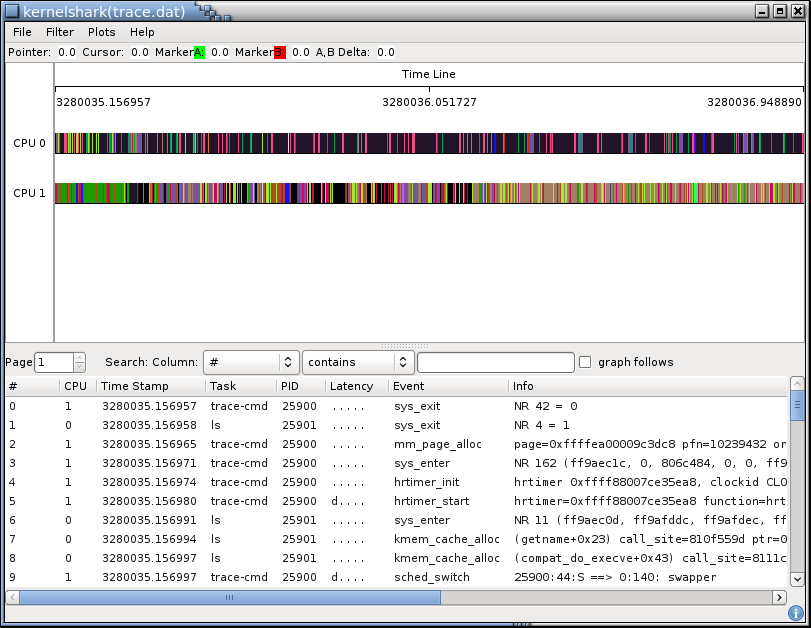
\includegraphics[width=5in]{kshark-open.png}
  \caption{KernelShark consists of a graphical display of the programs running on a computer over time (top half of screen), as well as a tabular view of the same information, in the form of CPU events such as processes switching, waking, or sleeping (bottom half of screen).}
\end{figure}

KernelShark's major failing is that it doesn't provide any tools or methods to
make it easier to find anomalies, but simple displays the information in one
kind of view. For example, in order to utilize information about cycles, the
user must manually recognize where cycles start and end. Then they must manually
compare all cycles to each other to see if anything is different, by going back
and forth on the timeline KernelShark provides.

KernelShark has a poorly designed UI that does not function as
expected. The tabular view on the bottom of KernelShark is not searchable, nor
can the columns be sorted. All lists in KernelShark cannot be sorted, meaning
that if the user has hundreds of tasks running, they must look through a list
with hundreds of tasks to find the specific task they want. Additionally, zooming out on
KernelShark's visual timeline is uninituitive and confusing, even for veteran
users of the tool.

%Using only this visualization, it can be difficult to see where the cyclical
%deadlines for the programs begin and end, making it hard to find when something
%misses a deadline. In addition, the tabular display of the CPU events in the
%bottom part of the screen has minimal search functionality and the different
%columns of the table are not sortable. Individual timelines for tasks can be
%displayed below this main chart, but the menu to select a task does not have
%any searching capability and does not order the tasks in any discernible way.

\section{Project Goals} % May Lynn
Our goals for this project were to make it easier and faster for SpaceX engineers to find software problems by creating a tool that visualizes rocket data and highlights problem areas. We have created an improved user experience and provided more visualizations of the data than the old tool. We have called the tool that we created SpaceShark.

\chapter{SpaceShark}
\section{Design} %Everyone gets a part

  The SpaceShark tool is meant to make it easier for SpaceX engineers to find bugs. We
  accomplish this through a variety of pages that serve unique purposes, giving
  engineers many options in how they want to approach finding a problem. 
  An overview of the trace data is given on the first page that is displayed to a user, 
  and more detailed information can be found by going to the other
  pages, including overall statistics, a cyclical breakdown of tasks, task-specific information, and
  task-to-task comparisons. Through these pages we provide engineers the ability
  to easily go from viewing their data in it's entirety to viewing specific
  details of one or two tasks, and vice versa, while providing intuitive visual
  guidance on where anomalies might exist.
  
  Below we will describe the pages in more detail, including the purpose
  of each page and how they accomplish their respective goals. This will be
  followed by an example user work flow.

  \subsection{Node-Webkit and HTML} %Rachel
    At the beginning of the project, the team researched possible tools and
    technologies for creating our application. One possibility was simply
    extending KernelShark, the existing tool. After looking at the code for
    this, a large number of C files, we decided it would be easier to
    reimplement and extend it in something else; understanding the code base
    would take a very long time, and we felt other languages had better
    UI and charting libraries. We looked into Java UI libraries for
    desktop applications, as well as web-technology based charting libraries.
    During this research, we found node-webkit, which allows for
    HTML/CSS/JavaScript applications to be packaged and run as desktop
    applications with no reliance on the internet. As this allowed us to take
    advantage of many existing UI widgit and charting libraries that many team
    members were familiar with, we decided to take this route.

\subsection{Load File Page}

\begin{figure}[H]
  \centering
      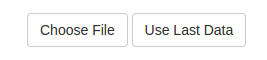
\includegraphics[scale=0.75]{loadFile-buttons.png}
  \caption{Choose File selects a new file and Use Last Data selects a file that has been previously been loaded into the tool.}
  \end{figure}

When the user first loads our tool, they will see the above screen in Figure 2.1. The purpose of the Load file page is to allow the user to choose which JSON file to load as their data, or choose to use the data that was previously used if this is not the user's first time using the tool. This allows the user to easily resume their work if they were previously examining a specific file.

KernelShark did not allow the user to use previously loaded data. SpaceX engineers often want to be able to save and revisit their work at a later time, so this served as an inconvenience to them. 

The code for the Load File page can be found in assets/js/loadFile.js.

  \subsection{Overview Page} 
  
  \begin{figure}[H]
  \centering
      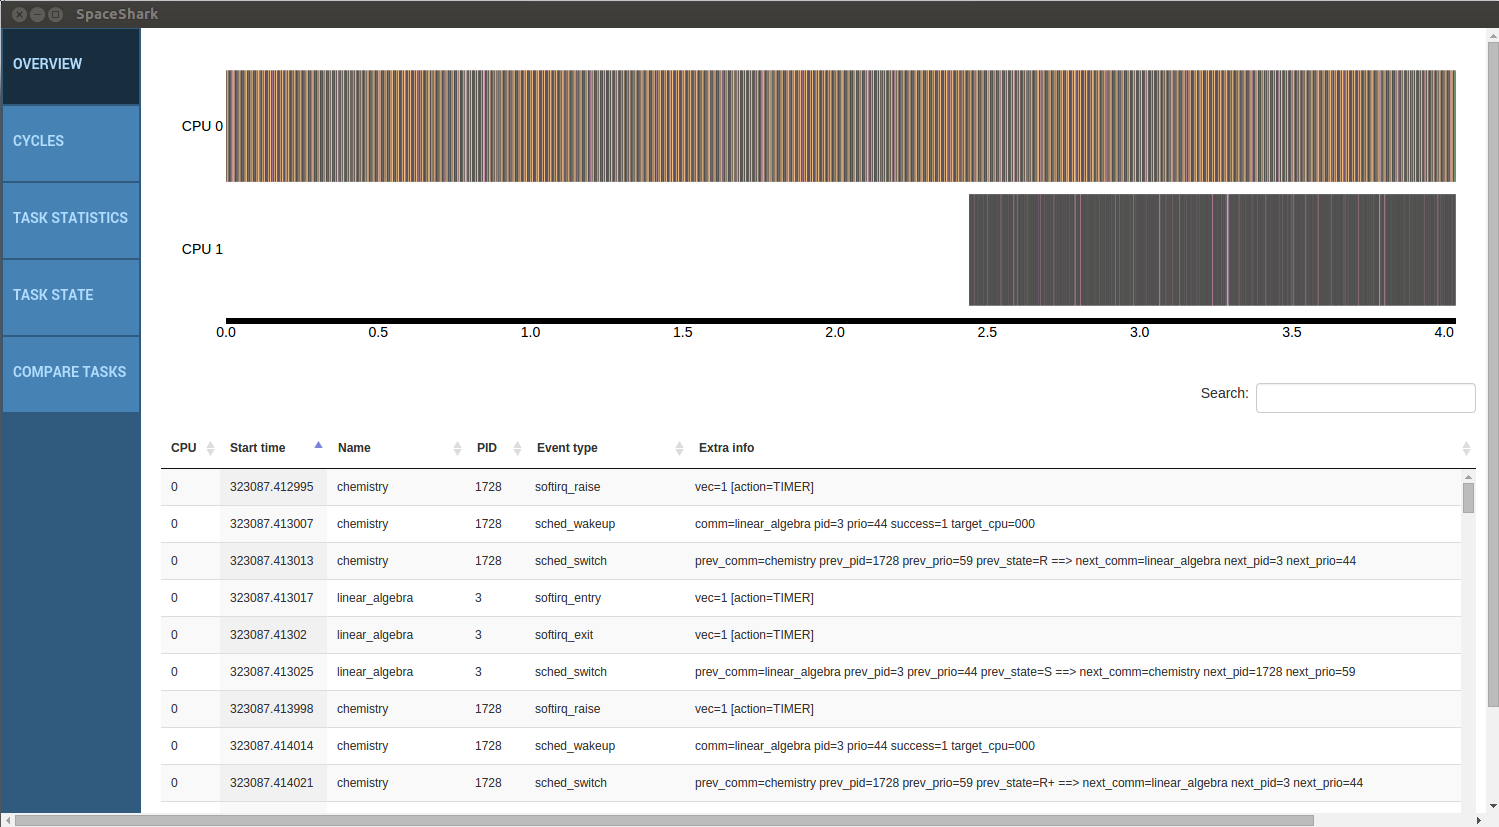
\includegraphics[width=5in]{overview-page.png}
  \caption{The top chart shows a graphical display of the programs running on the computer over time, and the bottom table shows a tabular version of this same information.}
  \end{figure}
  
The goal of the Overview Page is to be able to initially look at an overall view of the data, and then later be able to delve deeper into more specific details of the same data that are of particular interest to the user. More specifically both the graph and the table display the events list and through zooming, dragging, and clicking, we are able to find out more information about a specific event.

The goal of the Overview page is to be able to initially look at an overall view of the data, and then later be able to delve deeper into more specific details of the same data that are of particular interest to the user. More specifically the both the graph and the table display the events list and through zooming, dragging, and clicking, we are able to find out more information about a specific event.

    The code for the Overview Page is found within assets/js/main.js. This file is
    responsible for fetching and loading the data, creating a timeline
    visualization that the user can pan and zoom into, and creating a table that
    lists all events in the trace. The code for the chart and table is found in
    gantt-chart-d3.js and dataTables.scroller.js, respectively.

    The gantt chart plots all the CPU's grabbed from the loaded file on the same graph. It features both double click zooming and mouse scroll zooming and panning. KernelShark also had graph plots of the CPU's and included similar features as our tool though implemented in different ways. A user could zoom by clicking and dragging a rectangular box, from left to right, over the graph. This allowed the user to precisely view a specific area of the graph that they wanted. Although this zoom functionality seems helpful, it didn't really follow common zoom functionalities of a modern day desktop application. Zooming out of the graph in KernelShark is also unintuitive; the user can click and drag a rectangular box, from right to left, over the graph. This zooming out technique does not give the user any kind of information about how much the graph is zooming out and can therefore be very confusing to users. KernelShark is a responsive tool, partly because it doesn't load all the data while zooming. When zooming on KernelShark, a horizontal bar appears at the bottom of the graph to be able to easily pan. To save on resources, KernelShark doesn't load all the data from the beginning and the end of the trace file when zooming. 
    
    Users can click on a specific point in the graph and the table will update its position and jump to that event. KernelShark had this same functionality of being able to click on a spot in the graph and have the table display that event. %% IS THIS TRUE?!?!
    
    The user can also hover over any part of the gantt chart and be able to view a text box with more information about that particular event, such as the task name, the CPU it's running on, its PID, duration, and extra info. This is a feature that also existed in KernelShark, and we felt that it would be useful to reimplement in our own tool.

%% Use single click in this section, but need to eventually change our tool to use double click instead!!
%% Need to include more information about what specific search functionalities didn't exist in KernelShark?
    The columns of the table consist of the CPU, start time, name, PID, event type, and extra info about a particular event. By default, the table is displayed in ascending order from the first events start time to the last events start time. Hovering over any of the table cells highlights that entire row. Users can also click on a event to be redirected to that task on the Task State page. The search feature does multi-column filtering based on the search input. All columns headers are clickable to be ordered in ascending or descending order. Below the table, it shows the total number of entries and the range of entries that the user is currently viewing. KernelShark also had a list of events on the bottom half of their tool. It included more columns, such as latency and the event number it was from the trace file, but we felt that these columns were not helpful in including in our own tool. KernelShark gave users the option to search and filter our events in the table view, but it did not always yield correct search results. 
    
    In KernelShark, the user is able to look at a list of tasks with checkboxes and be able to individually plot them on the same graph as the CPU's. To maximize space on the Overview page, we decided to move this feature to its own page, which will be talked about in Section 2.1.7 Compare Tasks. 
    
    KernelShark was also able to give the user the option of displaying certain CPU's instead of all of them at once. We felt that this feature was not necessary because trace files that are used at SpaceX generally only have two CPU's , which is not a problem in terms of page space on the Overview page.
    
    KernelShark's main interface looks very similar to the Overview Page, but did not perform the same functionality that our tool does, such as correctly filtering and searching for events.
    
  \subsection{Cycles Page} %Alix

  \begin{figure}[H]
  \centering
      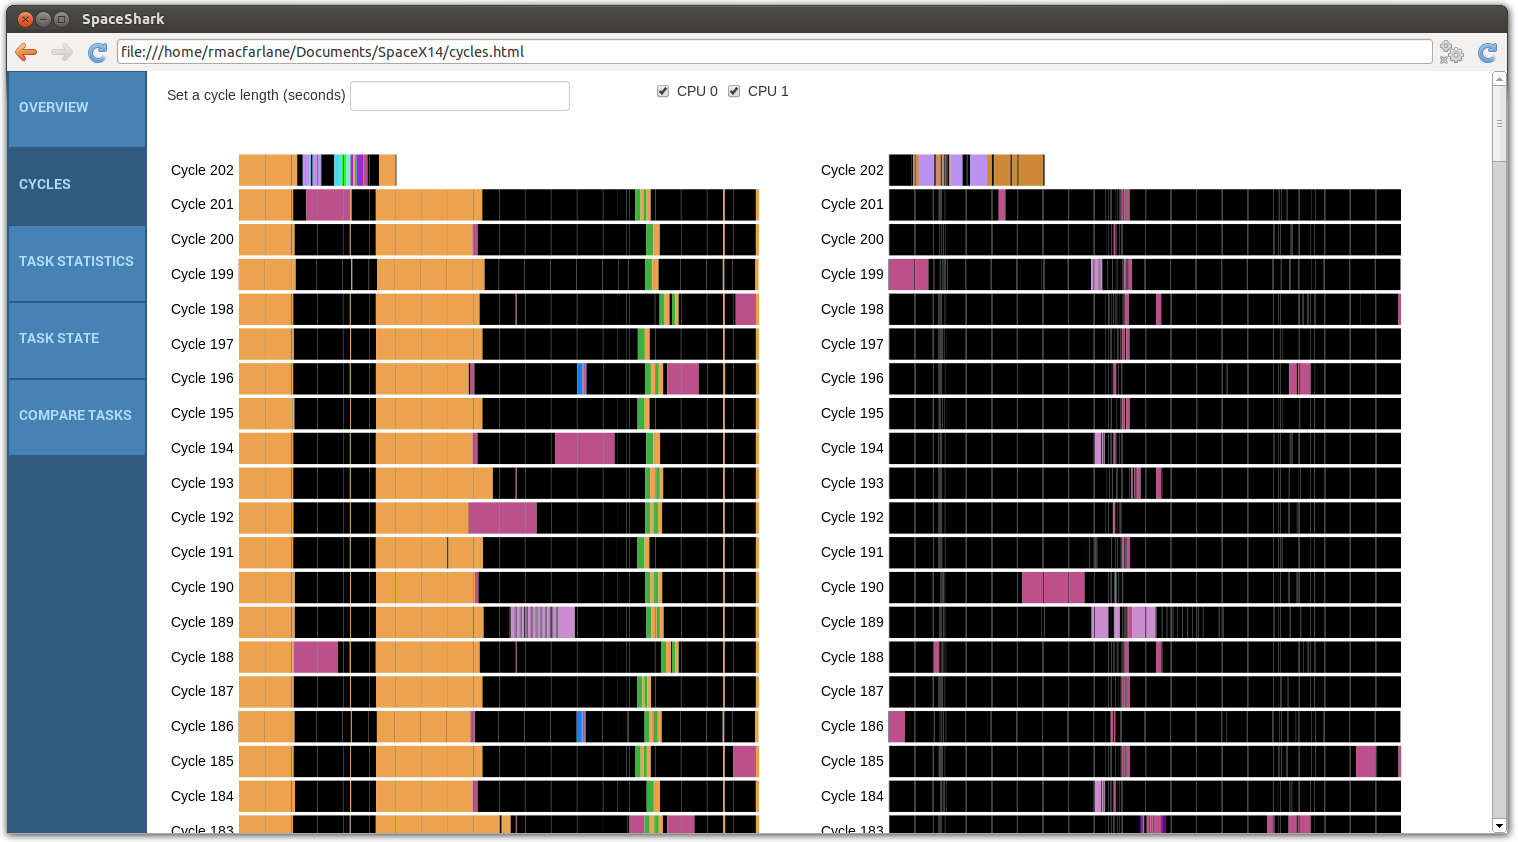
\includegraphics[width=5in]{cycles-page.png}
  \caption{The Cycles page displays graphs of each CPU. The user is allowed to
  input their own cycle intervals using the box in the top left. The checkboxes
at the top allow the user to toggle which CPUs display.}
  \end{figure}
  
  As tasks run in cyclical patterns on SpaceX rockets, being able to compare
  across cycles is very important to find strange behavior. The Cycles page
  breaks the data into cycles and stacks them, allowing a user to easily scan
  down this chart.

    The code for the cycles page is within assets/js/cyclesPage.js. This once again
    uses gantt-chart-d3.js to create the visualization after fetching the data.
    The page also has buttons to toggle on and off different CPUs, which removes
    or adds charts for these CPUs, rescaling other charts to use the full window
    space. Cycles are precomputed if print events exist within the trace. If
    not, the page will be blank when it first renders. The user can enter a
    number in the top box to set the period of desired cycles, which will then
    display a chart of cycles of that length. This feature also works even if
    print events are present in the data. On SpaceX rockets, the period of a cycle 
    is the same across CPUs, so entering a number at the top applies the change
    to all currently displayed charts.
    
    Zooming in and out works exactly like as on the Overview page. All CPU graphs are contained in one single .svg file, which is why the zooming works simultaneously over both graphs.
    
    The Cycles page did not exist in KernelShark. In addition, KernelShark did not give users the option of breaking the main graph into cycles.
  
  \subsection{Task Statistics Page} %May Lynn

  \begin{figure}[H]
  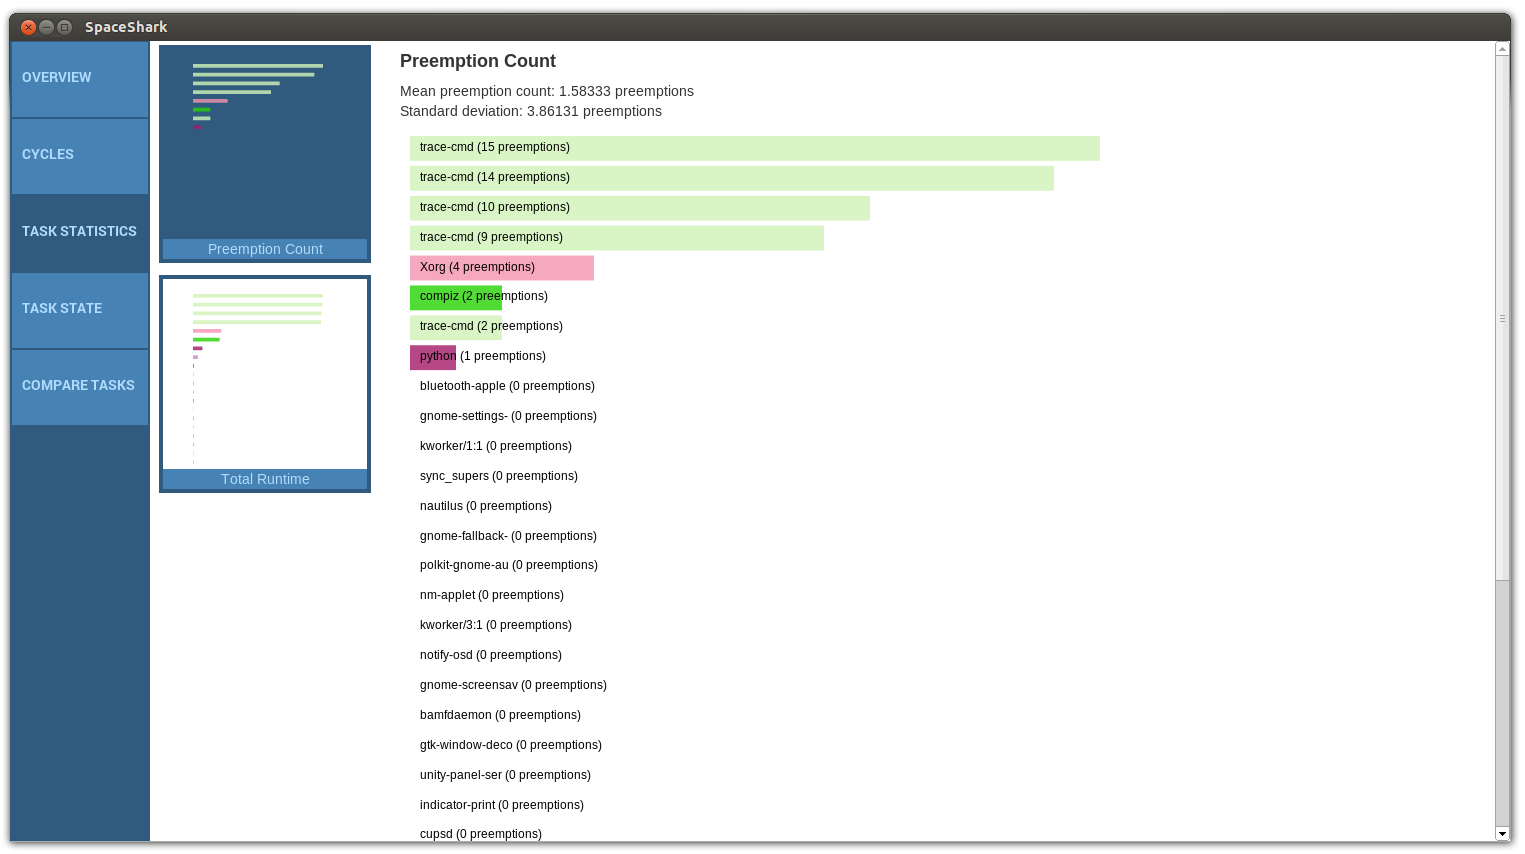
\includegraphics[width=5in]{task-statistics-page.png}
  \caption{The left column allows the user to navigate the bar charts, while
    also serving as a quick thumbnail view of each one. The right side displays
  the bar chart in a larger, more detailed view.}
  \end{figure}

The purpose of the Task Statistics page is to give an overview of the preemption count and runtime of each task. The page displays bar charts of the preemption count and runtime for each task, sorted from highest to lowest, as well as the averages and standard deviations of each. This makes it very easy to see if there are any outliers with a large number of preemptions or a long runtime, or to check if a task is behaving as expected.

The code for this page is within assets/js/preemptionChart.js and assets/js/runtimeChart.js. The bar graphs use the dc.js dimensional charting library.

All bars in the bar graph have distinct colors to differentiate tasks. The user can click on any task within the bar graph and will be redirected to the Task State page displaying more information about that task. KernelShark did not do analyze and manipulate trace data, so it did not include any task statistics. 

  \subsection{Task State}

  \begin{figure}[H]
  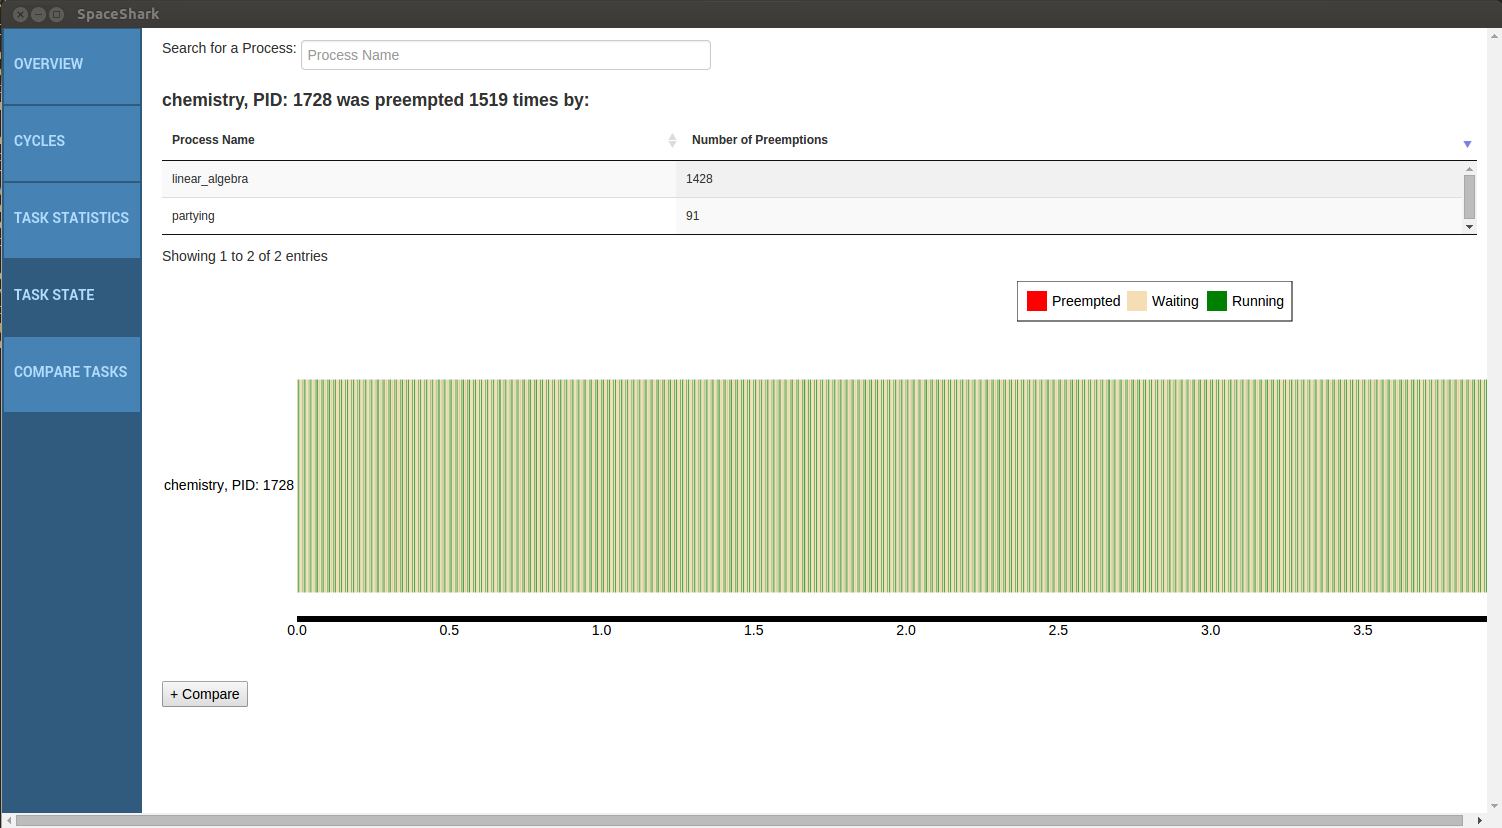
\includegraphics[scale=0.25]{task-state-page.png}
  \caption{The top of the Task State page displays a navigable table of tasks
  that preempted the current task. The bottom half is a graph representing the
state of the current task over time. The three possible states are preempted,
waiting, and running.}
\end{figure}

    The Task State page display information about a single task. The user is
    able to see interactions between other tasks and this task with a table of
    preemptions. Users can jump to tasks that preempted the current one by
    clicking on a row in this table. Additionally, the task's state over time
    is displayed at the bottom. Possible task states are preempted, waiting, or
    running and labeled with the colors red, beige, and green respectively. 
    The graph on the bottom half of the page functions the same as the graphs on the Overview (Section 2.1.3), Cycles (Section 2.1.4), and Compare Tasks page (Section 2.1.7). The user can click the ``+ Compare'' button at the bottom to add this task graph to a series of side-by-side graphs for comparison, which
    is described in Section 2.1.7 Compare Tasks.

    The code for this page is within assets/js/process.js. This page uses
    gantt-chart-d3.js for the chart and dataScroller.js to create the table of
    preemptions. The search box autocompletes task names using Twitter
    Typeahead.
    
    One of the main downsides of KernelShark is that it did not give the user the option to look at the data on a task level. Being able to look at specific tasks and see how many times a given task preempted other tasks is a very important feature to SpaceX.
  
  \subsection{Compare Tasks} %Wendy
  
  \begin{figure}[H]
  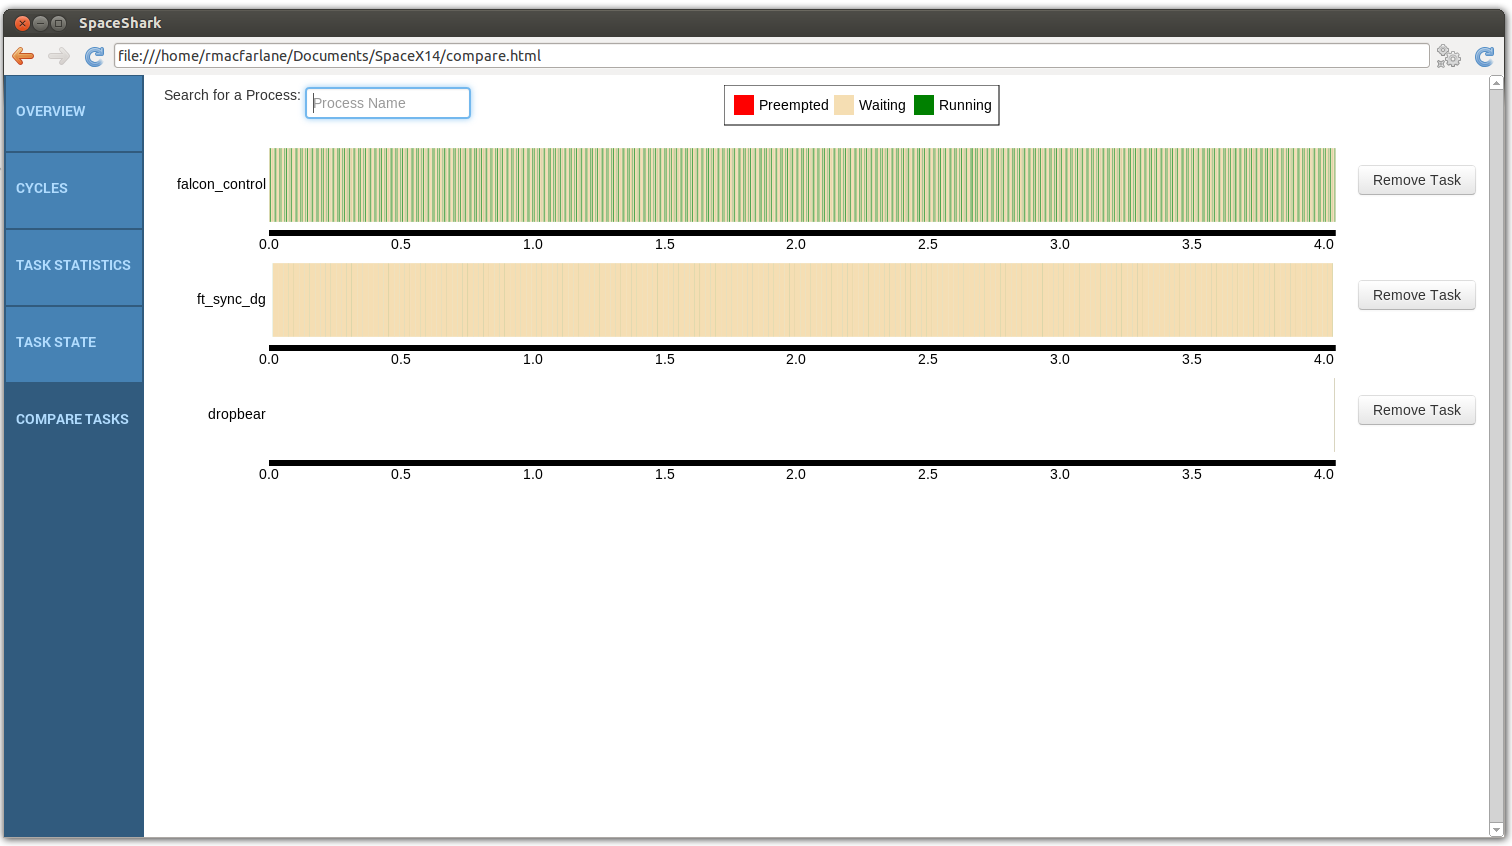
\includegraphics[scale=0.25]{compare-page.png}
  \caption{The Compare page vertically displays the Task State graphs for
  multiple tasks. They can be added, reordered, or removed all from this page.}
  \end{figure}

The Compare Tasks page allows users to view the same graph as the Task State
page, but for multiple tasks. Tasks can be reordered so that specific tasks can
be compared side by side for the same time period. This provides similar
functionality as the Task State page but with the additional benefit of
comparisons between tasks. This makes it simple to examine interactions between
two or more tasks. Users can plot graphs by either typing in a task name at the top of the page, or first viewing that task on the Task State page and clicking the "+ Compare" button. In both cases, the user can start typing in the text box and then will be given a list of possible task names that they might be interested in.

The code for this page is within assets/js/process.js. This page uses
    gantt-chart-d3.js for the chart, and draggabilly.js and packery.js to make the rows of graphs rearrangable.
    
    In KernelShark, the user is able to view a list of tasks and select which ones they want to graph. These selected graphs were plotted on the same graph as the CPU's, as stated before in Section 2.1.3. CPU graphs are too general to be compared with specific task graphs, so plotting these graphs on different pages seemed like a logical idea. Our tool has the added functionality of being able to easily remove task graphs by clicking the "Remove Task" button. The user can start typing in a name of a task, and then see a list of possible tasks based on user input. This is much faster and easier than going through a long list of tasks.
    
\subsection{Example User Flow}
  It should be noted that the SpaceX debugging process involves several steps,
  and an engineer likely has an inkling that tasks are not running in the
  pattern expected before taking a trace. Users will navigate through the tool
  differently depending on what level of information they already have.

  For example, if a user already has a hunch that a particular task is involved
  in the problem, they could immediately navigate to the Task State page. From
  this, they are able to see if the task preempted or was preempted by anything
  at an unexpected time. These related tasks are displayed in the table of
  preemptions, or on hovering over a preemption event on the graph below it.

  If a user does not have any suspicions about what happened, they could instead
  navigate to the Cycles page. By comparing the patterns of tasks run during
  different cycles, it should be easy to see an abnormal sequence of tasks. The
  user can then hover over this sequence on the chart and read which tasks are
  running. A user might also navigate to the Task Statistics page to quickly see
  if any task is being preempted far more than expected. This task could then be
  searched on the Task State page, as described above.

  There are many other possible ways users might navigate through the
  application, but the team believes the Cycles page and Task State page will
  prove especially useful.

\subsection{Selection of Graphing Tool} % Rachel
  Many pages render a timeline of running tasks which users can interact
  with by panning and zooming. This chart is critical, as a bug manifests
  itself as a task running at an unexpected time, or failing to run at a
  particular time. We spent several weeks experimenting with different
  javascript charts, including timeline.js, vis.js and gantt-chart-d3.js,
  to find one that would be suitably fast and easy for us to add new
  features to. Our main selection criteria were speed, zooming and dragging
  capabilities, and either built-in or easy to add handlers for user clicks
  on portions of the chart. We decided to use gantt-chart-d3.js because it
  rendered more quickly and was more responsive than the other charts. It
  also came with dragging capabilities, and the team saw that hovertext and
  click handling could easily be added. Zooming on d3 charts should be
  available out of the box, but did not function as expected because our y scale
  is ordinal rather than numeric and should not be rescaled. The team
  ended up writing a custom zoom function to handle this and other issues
  associated with syncing the zoom level of  multiple charts on the same page.


\section{Architecture} % Wendy

  \subsection{Overview}

  Our application has three main portions: the raw input, the parser,
  and the web-based desktop application. The sections are modular, and
  as long as output/inputs remain the same, internal changes to one section will
  not affect the other at all. Below we will discuss in more detail how each
  section works and how they relate to come together as our final application.
  Figure 2.7 provides a visual representation of the flow of our application
  while also displaying its modular parts.
  
  \begin{figure}[H]
    \begin{center}
  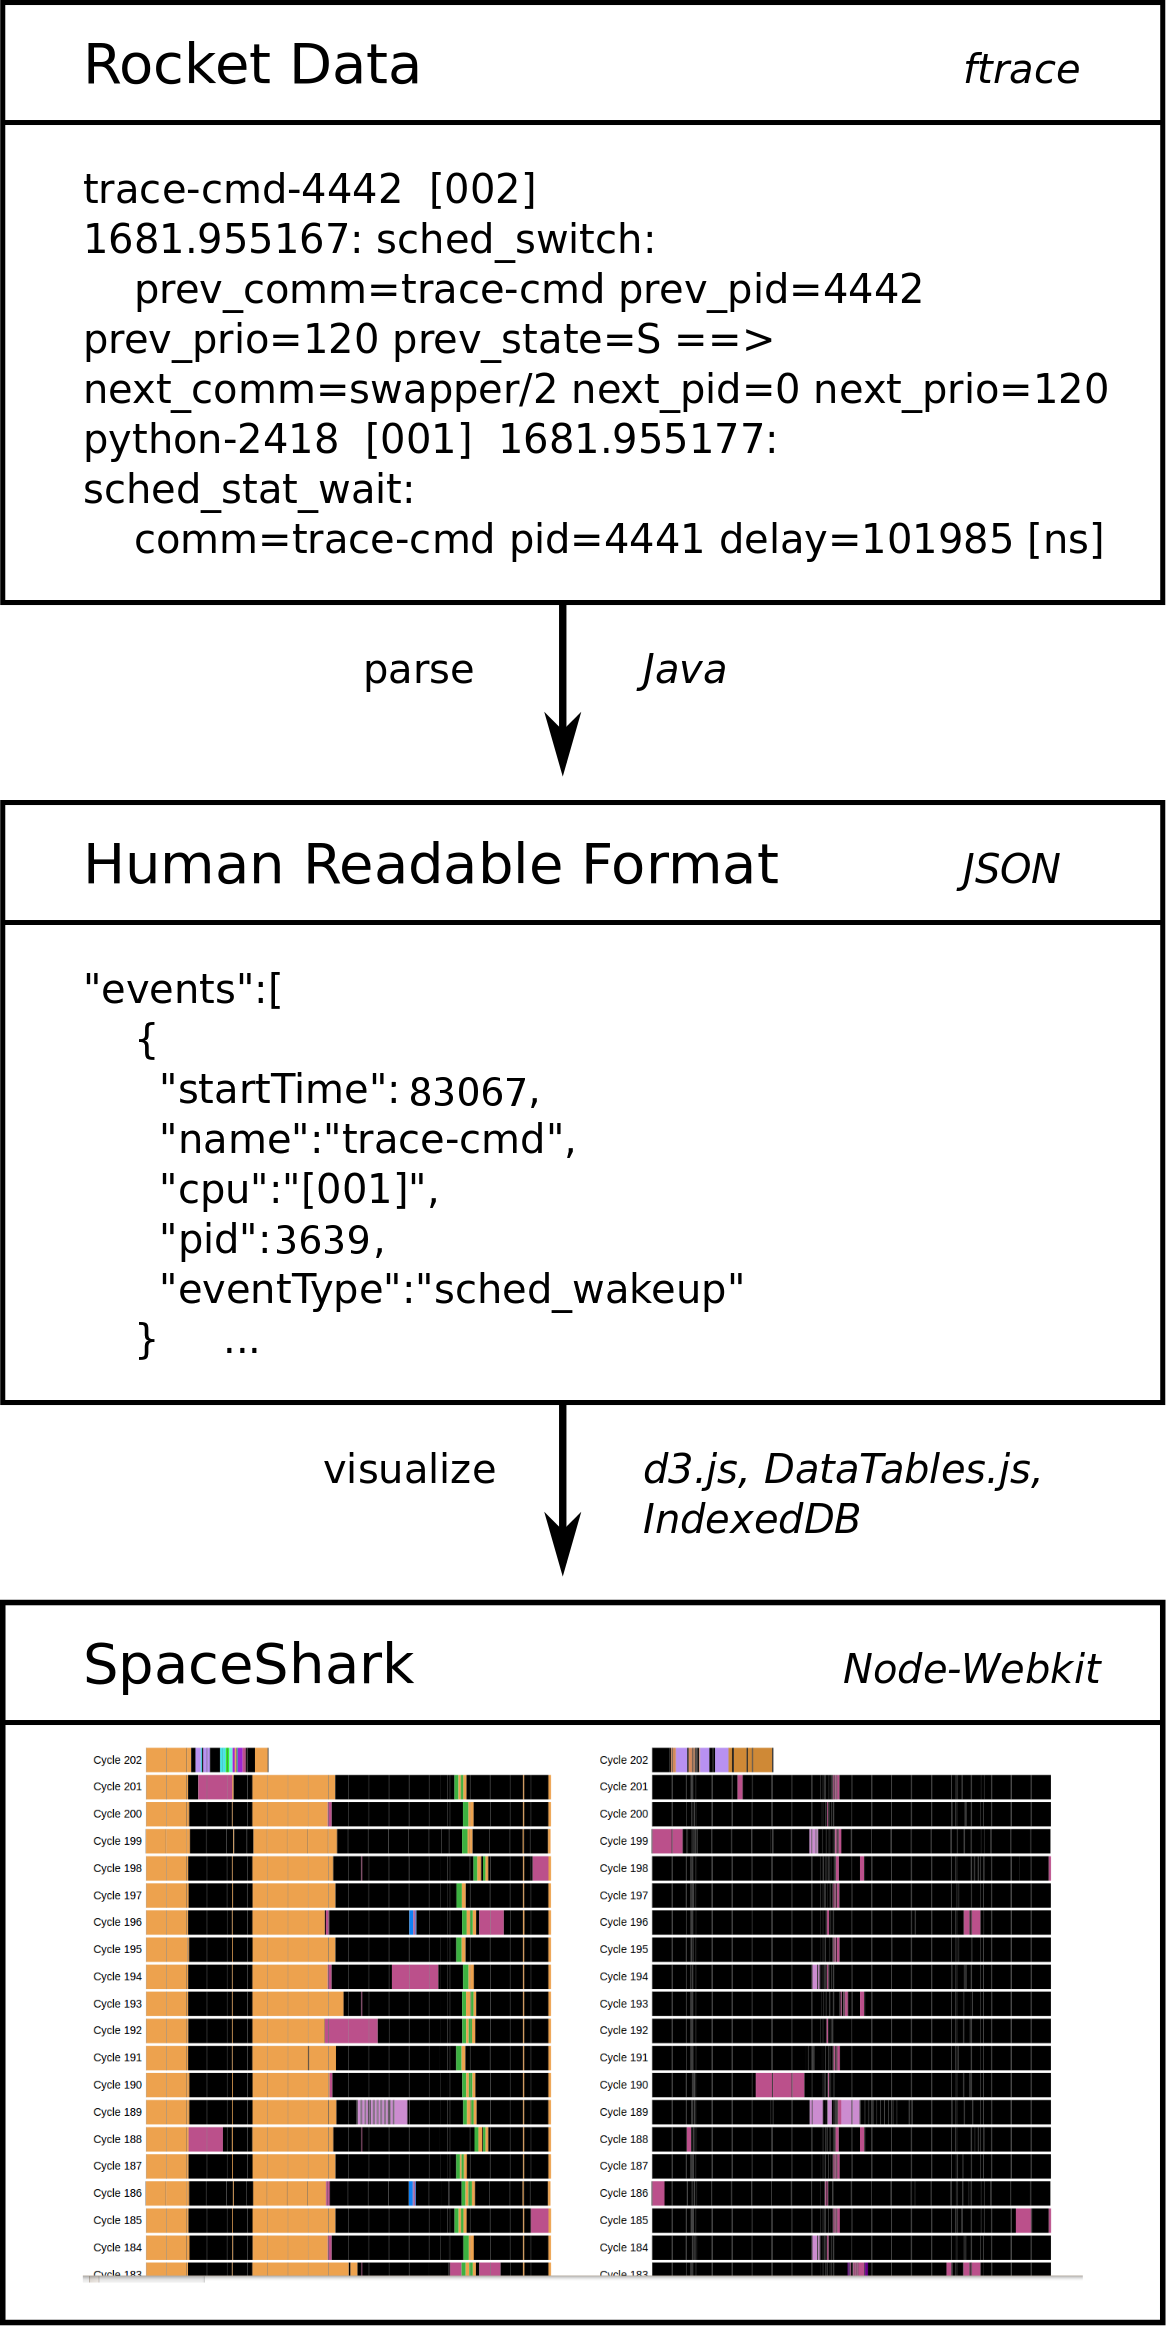
\includegraphics[scale=0.18]{architecture_diagram.png}
  \caption{A visual representation of three portions of our application. Each
  piece flows into the others while remaining modular, coming together to make our final tool.}
\end{center}
\end{figure}

  \subsection{Trace-cmd}

  Data is collected using a command-line utility called trace-cmd.
  trace-cmd records various events in the Linux kernel while it runs and then
  outputs this information into a data file with a particular binary format.
  trace-cmd is a powerful tool and can be used to trace many different types of
  events. The type of events recorded are specified by the user when they run
  the tool. Our goal is to help visualize scheduling data: what tasks were
  scheduled to run, wait, and migrate between CPUs over the time of the trace.
  We therefore assume that the user has taken a trace that captures scheduling
  events.

  Besides outputting data in binary format, trace-cmd also has a ``report``
  option, which takes an existing trace file and generates a human readable
  report of this record. An example line from a report is shown below.
  
\footnotesize\begin{verbatim}<idle>-0   [002]  2296.990243: sched_wakeup: comm=nautilus pid=2390 prio=120\end{verbatim}

\normalsize
  Using this format as a starting point instead of the
  raw binary format simplifies parsing.  We decided to leverage trace-cmd report
  instead of wrestling with the binary data ourselves. This allowed us to make
  progress faster and to avoid working on an already solved problem.

  The downside of this is that the format of the file generated by trace-cmd
  report is dependent on the version of trace-cmd used. To be able to reliably
  parse data and add additional information about preemptions, we need our input
  data to have a consistent format. This creates a dependency on a particular
  version of trace-cmd. The team has chosen to use trace-cmd version 2.2.1, 
  the same version that our liaisons currently use.

  \subsection{Parser}
  Next the parser takes in this raw data, and ultimately outputs the data
  reformatted into JSON with additional information. The file format of
  trace-cmd report is simple and consistent. The first line in the file
  gives a version number of trace-cmd report, and the second the number of
  CPUs in the captured trace. Each line in the remainder of the file is a
  single recorded event with a number of fields separated by whitespace.
   
  \begin{figure}
  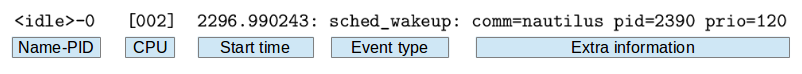
\includegraphics[scale=0.4]{parserExample.png}
  \caption{An example line of raw input, with the specific pieces labeled.}
  \end{figure}

  These five fields appear for every event, but the content of extra information
  varies based on the type of event. The units on the time stamp of the event,
  start time, are milliseconds since kernel boot.

  To parse these event lines, we read our file line by line and break on
  whitespace. Then it is easy to extract fields one by one. To deal with the
  extra information field at the end, we case on event type. Switch events
  are the only types of events that contain extra information that we need.  The
  extra information field of switch events gives the name, PID, and priority of
  the task being switched in for the currently running task. Importantly, it
  also contains a flag that indicates if the task being switched out transitions
  to a runnable or sleeping state. If the task is switched out and into a
  sleeping state, it has been blocked, which means the event is a preemption.

  The parser also calculates the total runtime of each task by looking for
  ``sched\_stat\_runtime'' events. These events give the time elapsed between
  a task being switched in and out of a processor, so by summing them for 
  each event, we are able to add a field to a task giving total runtime.

  The output is formatted as a JSON file, so that we can easily transfer it to
  the web application. The output JSON has the following elements:

  \begin{center}
    \begin{tabular}{|l|l|}
      \hline
      Tasks      & An array of all tasks seen in the trace\\
      \hline
      Events     & An array of all events seen in the trace\\
      \hline
      cycleEvents & An array of cycle events generated from user markers\\
      \hline
      numCPUs     & Integer, how many CPUs were in the trace\\
      \hline
      AutocompleteNames & An array of strings, listing all tasks names\\
      \hline
      AutocompleteEventTypes & An array of strings, listing all event types in
      the trace\\
      \hline
    \end{tabular}
  \end{center}

  As noted, several of these JSON objects contain other JSON objects: tasks,
  events, and cycleEvents. A task has the following data.

  \begin{center}
    \begin{tabular}{lll}
      Task      &        &                                        \\
      \hline
      Field           & Type         & Additional description \\
      \hline
      name            & string       & \\
      pid             & int          & \\
      events          & int array    & Indices into the Events array to find associated events\\
      preemptedBy     & string array & Names of tasks that preempted this task \\
      preemptionCount & int          & A running total of times this task was preempted                    \\
      totalRuntime    & long         & Time this task ran in milliseconds during the trace        \\
      totalWaittime   & long         & Time this task waited in milliseconds during the trace     \\
      totalSleeptime  & long         & Time this task slept in milliseconds during the trace     
    \end{tabular}
  \end{center}

  An event contains the data in the table below. Switch events contain some additional
  information. The switch event itself belongs to the task that is being
  switched out, but from the extra information field we also note which task
  was being switched in.

  \begin{center}
    \begin{tabular}{lll}
      Event      &        &                                        \\
      \hline
      Field     & Type   & Additional description                 \\
      \hline
      name      & string &                                        \\
      pid       & int    &                                        \\
      cpu       & int    &                                        \\
      startTime & double & Time in milliseconds since kernel boot \\
      eventType & string &                                        \\
      extraInfo & string &                                        \\
      \hline
      Switch event specific data & & \\
      \hline
      activeName & string & The name of the task switching in      \\
      activePID  & string &                                        \\
      \hline
      Print event specific data & & \\
      \hline
      userMark   & string & Currently unused
    \end{tabular}
  \end{center}

  trace-cmd can also pick up ``print'' events. Print events allow users to add
  their own markers as a task runs. A user can generate a print event by making
  an addition to the code of a task. We rely on these user-generated markers to
  identify cycles; print events occur periodically in some of the tasks we are
  tracing. Print events can also be used for other purposes, so we check to see
  that the user has annotated them with ``CYCLE\_START'' by looking at the extra
  information field of a print event. If the extra information field starts with
  ``CYCLE\_START'', then we create a cycleEvent that contains the following data.

  \begin{center}
    \begin{tabular}{lll}
      cycleEvent      &        &                                        \\
      \hline
      Field     & Type   & Additional description                 \\
      \hline
      startTime      & double &                                        \\
      extraInfo       & string    &                                        \\
    \end{tabular}
  \end{center}

  To see an example, view Appendix A at the end of the report.
  \newline
  \newline
  As long as this file remains the same, any changes to the internals of the
  parser will not affect the application itself. Additionally, this will allow
  someone with a different output to write their own parser to create the same
  type of output so that they can view their data in our tool.

  \subsection{Web Application}

  \subsubsection{IndexedDB}

  The application takes the JSON file and loads it into IndexedDB, a
  browser-based database. IndexedDB is built into most browsers, including
  node-webkit, which actually runs Chromium. More information on the details of IndexedDB can be found here:
\begin{center}
  https://developer.mozilla.org/en-US/docs/Web/API/IndexedDB\_API
\end{center}
  We use IndexedDB to store data between pages. It also
  maintains storage between application sessions. Therefore, we are able to have
  the choice to load the same file again, without reselecting it. If the user
  chooses to load a new file, we just write over this.
  Specifically, we store 
  \begin{itemize}
    \item numCPUs (number of CPUs for this file)
    \item cycleEvents (the events divided into cycles for the cycles page)
    \item Tasks (a list of all the tasks with various information)
    \item AutocompleteNames (used for autocomplete in search bars)
    \item AutocompleteEventTypes (also used for autocompleting)
    \item Events (a listing of all the events)
  \end{itemize}
  These correspond to the JSON types laid
  out in the Parser section (presumably we have numbers/pages later).

  Using the node-webkit profiling tool, we can see that IndexedDB is the slowest
  part of our application, as transactions with the database must be opened and
  closed. Ideally, we would use something less complex, but other options such
  as Local Storage did not have enough space for our large files.

  IndexedDB also has  a size limit, but this is typically not reached except for
  unusually long files or files with 4 or more CPUs. Our liaisons have indicated
  that the trace files they deal with do not exceed 4 CPUs.

  \subsubsection{Local Storage}

  Our application also makes use of Local Storage, another tool
  built into most browsers and node-webkit. This is a small and quick to access
  storage method. We primarily use it to save state between pages, notably
  display states. One example is the zoom level of the graph, which does not
  change between loads of the same page. Local Storage is also retained between
  application sessions. Similarly to our IndexedDB data, if the user chooses to
  load the same data we still have their state changes saved. If they load a new
  file Local Storage is cleared.

Here is a list of the Local Storage variables that we are using, and what they are for:
\begin{itemize}
\item cellData: A string containing the name and PID of the task currently being
  shown on the Task State page. 
\item compareCurrScale: The last recorded scale for the Compare Tasks graphs.
\item compareCurrTranslateX: The last recorded x translate for the Compare Tasks
  graphs.
\item compareCurrTranslateY: The last recorded y translate for the Compare Tasks
  graphs (not used).
\item compareData: A list containing strings with the names and PIDs of the
  tasks currently being shown on the Compare Tasks page.
\item cyclesCurrScale: The last recorded scale for the Cycles graphs.	
\item cyclesCurrTranslateX: The last recorded x translate for the Cycles graphs.
\item cyclesCurrTranslateY: The last recorded y translate for the Cycles graphs
  (not used).
\item displayedCPUs: A list of the CPU numbers that are being displayed on the
  Cycles page.
\item firstEventTime: The time that the first event occurs, non-normalized.
\item hasEverExisted: We check this variable to see if there is content in Local Storage so that we know whether or not to give the user an option to use their previous data on the Load File page	
\item mainCurrScale: The last recorded scale for the Overview graph.	
\item mainCurrTranslateX: The last recorded x translate for the Overview graph.
\item mainCurrTranslateY: The last recorded y translate for the Overview graph
  (not used).
\item maxDuration: The longest time in seconds that a CPU ran for. Serves as
  the end time for all graphs.
\item processCurrScale: The last recorded scale for the Task State graphs.
\item processCurrTranslateX: The last recorded x translate for the Task State
  graphs.
\item processCurrTranslateY: The last recorded y translate for the Task State
  graphs (not used).
\item tableScroll: Used by the Overview table.
\end{itemize}
DataTables also makes use of Local Storage in order to save the scroll position of the table.

  \subsubsection{Overall Application Structure}

  The general structure of our code is similar to
  most web applications. In the root we have HTML files, which call to
  JavaScript and CSS files, located in assets/js and assets/css respectively.
  HTML files do not have any JavaScript or CSS inside them, but exclusively call
  to other functions for this. Each page has its own specific JavaScript file,
  and then there are a number of shared files that multiple or all pages use. We
  have used a number of JavaScript libraries.
  \subsubsection{Creating a Timeline}
  On the overview, cycles, task state, and task compare page, the same type of
  chart is used. The chart shows either which task is running at a given time,
  or what state a process is in at a given time. The chart is fed a list of
  events to display and a number of optional settings before being drawn. The
  array of all events needs to be passed through several helper functions
  before it is ready to be given to the graph.
  
  \begin{enumerate}

    \item The events list is filtered to only contain switch events. Switch
      events are all that are needed to determine which task was running, or
      what state a task was in.
  
    \item All start times are normalized so that first event is at time zero.
      In the original events list, the start times of events are given in
      milliseconds since kernel boot, which is not relevant. We separate our
      events by CPU, and for each grouping of events, shift the start times
      so that the first one occurs at zero.
  
    \item The graph needs to know its time domain, so we calculate this
      endpoint. How this calculation is performed depends on which page we are
      on. On the overview page, we want to compare across CPUs. Each CPU may not
      be processing tasks for the entire duration of the trace. For example, all
      events on CPU 0 might take only 3 seconds, while all events on CPU 4 take
      4. We take the maximum of the total duration of events across CPUs, in our
      example, 4 seconds. The same calculation is used for the compare page so
      that the time range on the x-axis will be the same across all tasks.  On
      the cycles page, our time range is simply the length of a cycle.
  
    \item The gantt chart is passed its parameters in preparation to be drawn,
      not including the events. These parameters include the name of the page it
      is currently on, which will allow it to modify its behavior based on
      context, as well as what attribute to group by (CPU, cycle, or nothing).
      Width and height can also be passed, which allows charts on the compare
      page to take up little vertical space, while the overview page chart uses
      as much space is available to it.
  
   \item The events have their duration calculated, to determine how large each
     rectangle should be drawn. For example, on the main page we calculate the
     difference between the start times of consecutive switch events. This gives
     us the amount of time each task was running for.
  
   \item The gantt chart is passed the events and drawn, and the colors are set.
     The chart assigns a class to each task based on its PID, and we randomly
     select a color for this class and add a style tag to the page. Our random
     color selection is seeded so that the same colors will be assigned every
     time. We considered producing a stylesheet after parsing so we did not have
     to generate this each time, but in profiling the application we saw that
     this process was actually quick, and decided this change was very low
     priority.

  \end{enumerate}
  \subsubsection{Primary JavaScript/CSS files}
  One of the primary JavaScript files we've worked
  with and changed is gantt-chart-d3.js. This file is the logic for all of the
  graphs. This file was originally written by Dimitry Kudrayvtsev, but we have
  significantly modified it to produce the behavior we want.

  The chart takes in data and groups it by a particular attribute. Each piece
  of data, here, a scheduling event, is rendered as a rectangle. The
  length of the rectangle is determined by the event's duration, and its
  placement on the graph by its start time and group. Examples of groups are
  CPU or cycle.

  The chart assigns classes to each rectangle so that they can easily be
  colored (lines 259-279), and sets up a mouseover handler to display hover text
  over an individual event (lines 296-306). On the overview page, clicking
  on an event will scroll to it in the data table - this handler is set up on
  lines 291-295. Lastly, we added zooming behavior to the chart that is
  preserved on navigation. By using local storage as described on page 17, we
  are able to check that graphs added to the compare page will render at the
  same zoom level as others, and will zoom in sync with each other.

  To function properly, the chart needs a list of events passed to it to
  display, as well as a property to group on. Behavior on our pages varies
  slightly, so a parameter is also passed to indicate to the graph which
  page it is rendering on. This is either ``MAIN'', ``CYCLES'', ``PROCESS'',
  or ``COMPARE.'' ``MAIN'' and ``PROCESS'' refer to the overview and task
  state pages - these were the working titles we used through most of the
  semester.

  Sidebar.js is a fairly simple script that creates the sidebar for all of the
  pages, excluding the first page of the application, where the user chooses a file.
  It controls navigation and sets highlighting of the current tab.

  The other non-page specific files are mostly borrowed and unedited from
  JavaScript libraries, so for documentation on those you can visit their
  respective pages online.
\begin{itemize}
\item d3.js (d3js.org)
% d3 - http://d3js.org/
\item dc.js (dc-js.github.io/dc.js)
% dc - http://dc-js.github.io/dc.js/
\item Draggabilly (draggabilly.desandro.com)
% draggabilly - http://draggabilly.desandro.com/
\item Packery (packery.metafizzy.co)
% packery - http://packery.metafizzy.co/
\item DataTables (datatables.net)
% datatables - https://www.datatables.net/
\item Twitter Typeahead (twitter.github.io/typeahead.js)
% typeahead - https://twitter.github.io/typeahead.js/
\item Underscore (underscorejs.org)
%% FIXME - any more?
\end{itemize}

\section{Packaging and Distribution}
  Our code is publicly available on Github at
\begin{center}
  github.com/golden3point14/SpaceX14
\end{center}
The README of this repository provides a link to download a
  64 bit Linux version of the application. This release is a zip file that
  contains an executable, the parser, a short wrapper script, and two additional
  files that are necessary to get the executable to run: nw.pak and icudlt.dat.
  The short wrapper script is called spaceshark and has the following usage:

\begin{verbatim}spaceshark [-p | --parse filename] [-o | --open filename] 
           [ -h | --help]\end{verbatim}

  The first option allows the user to pass an unparsed trace file to the
  application. The parser will be run and output a JSON file, which will be
  passed to the application as it opens, skipping the load page that asks the
  user to choose a file. The second option allows the user to pass a parsed
  JSON file to the application. Finally, using the -h flag or any option
  not recognized by the script will display the usage and a description of
  available options.

  We also created a 64 bit release for Mac, which includes the parser but does
  not have a script to connect it to the application. As most developers at
  SpaceX use Linux machines, we decided that there were better uses of our time
  than providing releases for other operating systems.


\chapter{User Feedback} % Alix
\section{General Feedback} % Alix
During a week long site visit at SpaceX, we were able to user test with four SpaceX engineers. 
User testing played a major component in making sure that we were creating a
tool that the engineers would be able to use to find errors in their rocket
software. We found a few discrepancies between what we thought would be useful
for engineers and what engineers actually found useful. Additionally, we were
able to see which aspects of the tool had been done well and gain a better
understand of how these features helped SpaceX engineers. Overall, user testing
provided a good way to ground our project, by showing us what worked and what
did not, so that we could be sure our tool was useful and make decisions
accordingly. We will focus mostly on the negative feedback, as critical feedback
was the most useful in moving forward to improve the tool.

A common theme was that our tool was not cohesive. There wasn't enough
connection between the different sets of data our tool used. Context is
important to SpaceX engineers. The way a task behaves by itself isn't
enough to understand what is going on with the computer as a whole. Seeing the
interactions of the entire system is more useful than seeing the behavior of individual pieces.

Below we will cover our methodology, feedback for specific pages, and how that
feedback shaped
the changes we made, leading to the current version of SpaceShark.

\section{Methodology} % Wendy
In order to test our tool, two members of our team would watch an individual
work their way through it using our sample data, or in some cases the user's
data if they had some prepared. We tried to provide as little
input as possible, except for encouraging the team member to think out loud and
talk about what they were thinking, expecting, or doing, and why. While the user
did this, we would take notes on both what they were saying and what they were
doing.

Once the user felt like they had explored the tool, we talked more in-depth
about their experience, also elaborating on our intent with the tool,
encouraging explicit feedback on how we could make the tool better. A large
portion of this process went to brainstorming with the user and finding out why
a page was helpful or unhelpful for their specific workflow.

\section{Feedback on Specific Pages} % Alix

\subsubsection{Overview Page}

The main page of KernelShark featured a graphical display of the processes
running over time and a tabular version of the same information. KernelShark had
a number of problems, including poor user interface, unintuitive zooming,
features that did not work as expected, and a limited way to view the data.
Using KernelShark required the user to know the behavior they expected to see
beforehand, as it did not provide any indication of cycles or features aimed
specifically at detecting errors.

Before winter break, our tool featured a graphical representation of tasks running over time,
as well as three tables that displayed the top ten preempted, longest running, and
longest waiting tasks. 
Through user testing, we found that three out of four users mentioned that they
did not find the statistics on the Overview page helpful. Because only one user found the statistics useful,
we decided as a team that it would be best to omit them from the Overview page, and
only display them on the Task Statistics page.

Additionally, the Overview page initially only showed the graphical
representation. Two of the users mentioned that the typical workflow of the tool
would be to visually find the problem in the graph, zoom in to that particular
strange spot in the graph, be able to jump to that spot in the events list, and
then scan a tabular version of the events list. In order to have this workflow,
we would need to have the tabular version of the graph on the Overview page.
As a result we decided that the Overview page of our tool would have both the
graphical version of the time series data, as well as the tabular version of it.
This gives our Overview page the context that SpaceX engineers are looking for.
It is easy to find something interesting on the graph, and then get the details
on it via the tabular display.

\begin{figure}[H]
\begin{center}
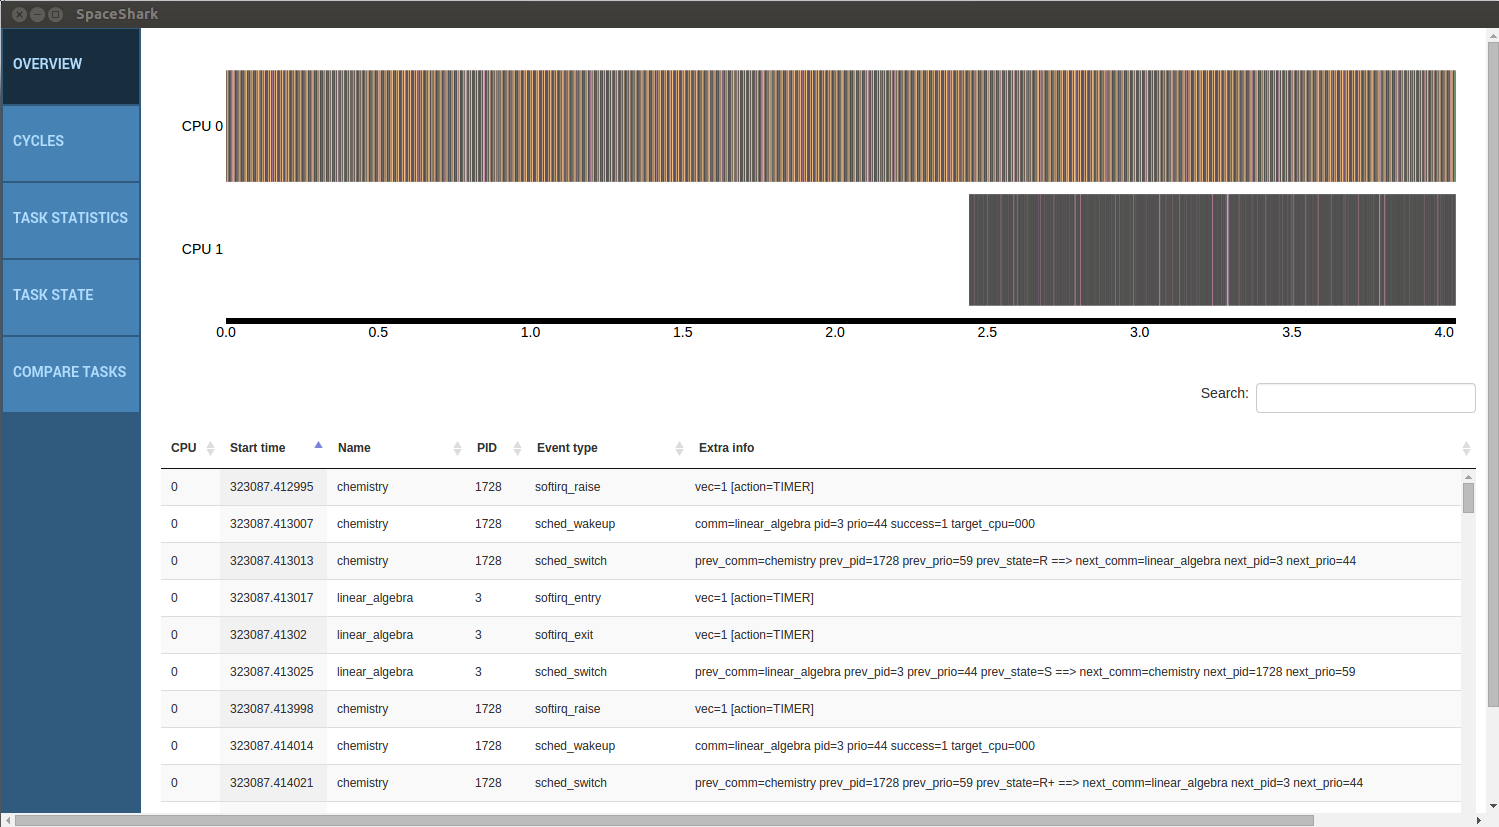
\includegraphics[width=4in]{overview-page.png}
\caption{A current screenshot of our Overview page. At the top is a graphical
representation of the tasks, and the bottom is a tabular view.}
\end{center}
\end{figure}

Our Overview page mimics the good
functionality that KernelShark had. Additionally, it allows users to filter the
tabular list of events on a variety of properties, and jump directly from a
specific point in the graph to the same point represented in the table. Double
clicking on a particular task in the table will also take the user to the
Process page, where they can get more information on a specific task. Covering
much of KernelShark's functionality on this page allowed us to use the rest of
our tool to surpass KernelShark's functionality and create a more versatile
tool.

\subsubsection{Task State Page}

With KernelShark, the user could pull out a graphical display of a single
task and put it on its own line. However, that was the extent of what
KernelShark did with regards to individual tasks.

We wanted to take this idea further by providing detailed information and
statistics about individual tasks. This would give users a different way to view
their data, which our liaisons thought would be helpful
in the debugging process.

\begin{figure}[H]
\begin{center}
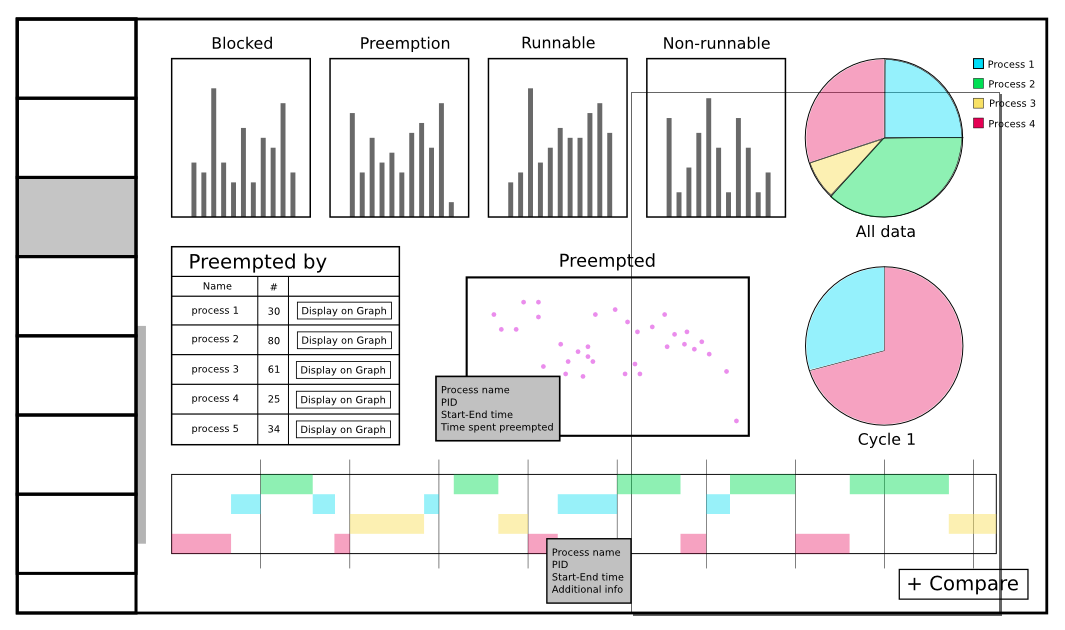
\includegraphics[width=4in]{perProcess-49.png}
\caption{The first mock-up we created for the Task State page.}
\end{center}
\end{figure}

Since there was no existing Task State page, we designed a mockup of it at the
beginning of the project. It features many different kinds of visualizations,
such as histograms of how long the task was in each state for, a scatterplot of 
what preempted it, a table of what preempted it, pie charts representing the 
data in cycles, and a graphical display of the time series data highlighting 
the process in the graph. Through user feedback with the liaisons, we found 
that our mockup included way too much information that SpaceX engineers would 
not have found useful. Since preemptions are generally
indicative of problems, we really wanted to focus on this on the Task State
page.

\begin{figure}[H]
\begin{center}
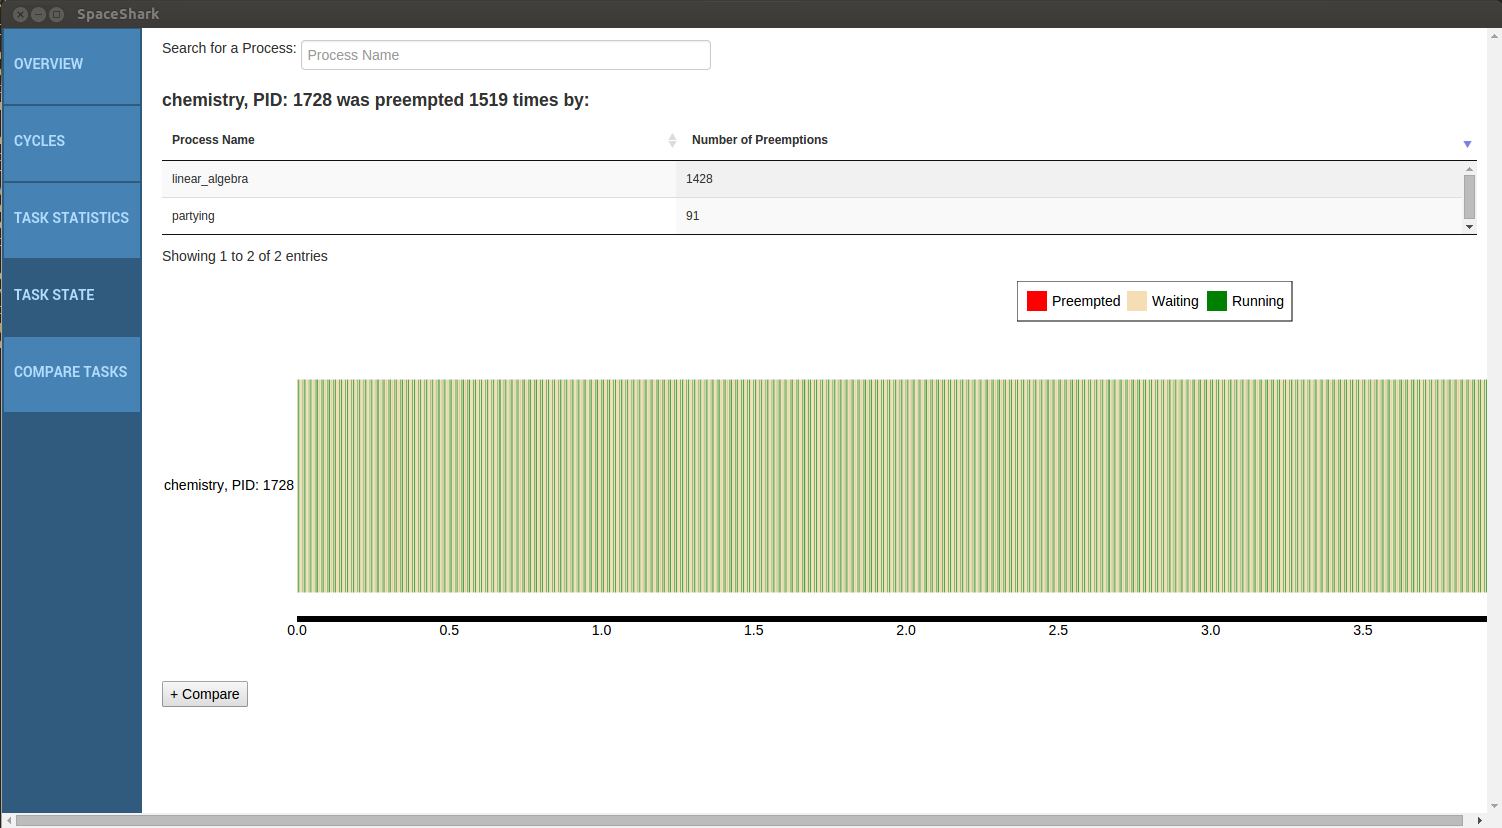
\includegraphics[width=4in]{task-state-page.png}
\caption{A screenshot of the current version of the Task State page. The three
colors indicate the three states a task can be in: running, waiting, or blocked.}
\end{center}
\end{figure}

On the Task State page, the user is able to type in a particular task, see
how many times it was preempted and which processes preempted it, as well as
view a graph showing how long it was in one of three states: running, waiting,
or preempted. This design has a minimalistic page view compared to the mockup,
but makes better use of the information it provides, and includes less
extraneous, unhelpful information.

This pages allows SpaceX engineers to find information on specific tasks, which
is something that KernelShark was unable to do. It helps engineers dig in to the
details, especially when used in conjunction with the broader context provided
on the Overview page and other pages.

When user testing, we received feedback that this page needed more context,
prompting us to create the Compare Tasks page. The Compare Tasks page has not
yet been user tested, but we hope it will meet this need by allowing users to
display multiple state graphs side by side to look at anomalies in context.

\subsubsection{Cycles Page}

One of the most notable things that separates our tool from KernelShark is that
KernelShark did not provide information about cycles, meaning that users had to
manually determine where cycles were.
The Cycles page in our tool lets the user easily find anomalies by splitting up
the Overview page graph visualization into cycles.

\begin{figure}[H]
\begin{center}
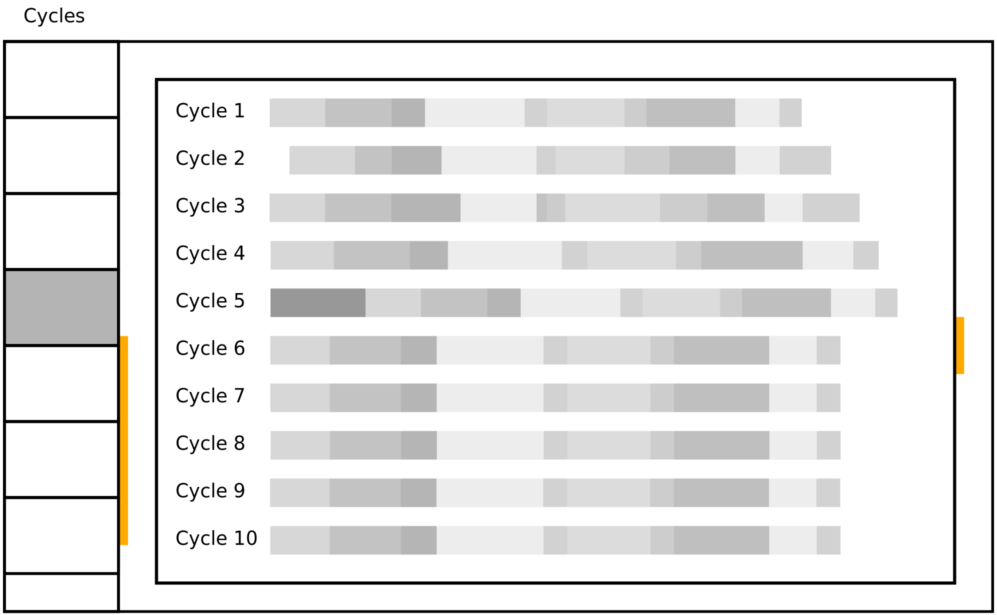
\includegraphics[width=4in]{oldcycles.png}
\caption{A mock-up of the Cycles page. Initially only one CPU at a time could be
displayed, as shown here.}
\end{center}
\end{figure}

We received nearly all positive feedback on the Cycles page, and this seems to
be the most useful aspect of our tool.

The first change  we made was very minor; rather than ordering the cycles from first cycle to last cycle, we changed it to be ordered from last cycle to first. We made this change because anomalies are normally found within the last cycle, which SpaceX engineers would want to see displayed prominently at the top of the page.

Additionally, this page initially relied on the user's code generating ``cycle
markers'', which meant that this functionality would not have worked with old
traces, or traces that didn't conform to our specific markers. One engineer
suggested that we add the ability to enter in cycle length and have it display
cycles based on that. We chose to implement this, taking this page from having
very specific requirements to being usable with any data.

\begin{figure}[H]
\begin{center}
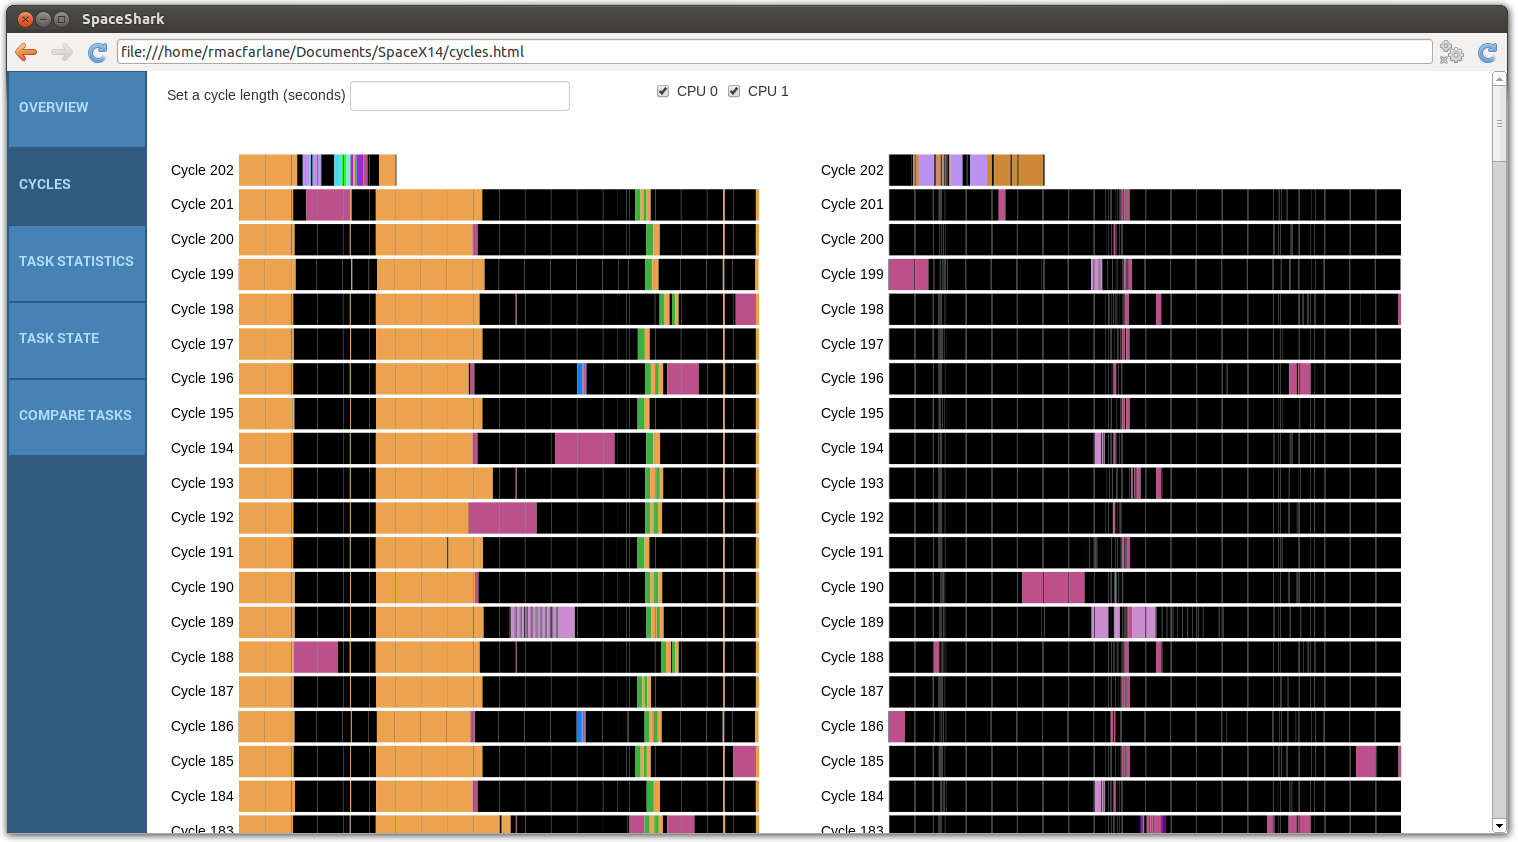
\includegraphics[width=4in]{cycles-page.png}
\caption{A screenshot of the current Cycles page. Multiple CPUs can be displayed
at once using the checkboxes at the top of the screen. The input box on the top
left allows users to choose their own cycle length.}
\end{center}
\end{figure}

%\chapter{Challenges}
%\section{trace-cmd versioning} % Rachel
%  As already described, we collect data using a command-line utility called
%  trace-cmd. trace-cmd records various events in the Linux kernel while it runs
%  and then outputs this information into a data file with a particular binary
%  format. trace-cmd also has a ``report'' option, which takes an existing trace
%  file and generates a human readable report of this record. Using this format
%  as a starting point instead of the raw binary format simplifies parsing.
%  We decided to leverage trace-cmd report instead of wrestling with the binary
%  data ourselves. This allowed us to make progress faster and to avoid working
%  on an already solved problem.
%
%  Unfortunately, the format of the file generated by trace-cmd report is
%  dependent on the version of trace-cmd used. For example, the formatting of the
%  ``extra info'' field of a switch event is liable to change. We use this
%  field to identify preemptions. To be able to reliably parse data and add
%  additional information about preemptions, we need our input data to have
%  a consistent format. This creates a dependency on a particular version
%  of trace-cmd. Our liaisons have been using trace-cmd version 2.2.1, so
%  our parser expects input data to be in the format of 2.2.1.
%\section{Selection of charting tool} % Rachel
%  We chose to use web technologies because we felt there was a wealth of
%  charting and UI/UX tools that we could use. We spent several weeks
%  experimenting with different charts for the main page. The main page renders a
%  timeline of running tasks, which is essentially a large number of colored
%  bars. This chart needed to be responsive to zooming and dragging, and to
%  dealing with click events to move to a particular time in the table of events
%  displayed below it.
%\section{Speed} %Wendy
%The data SpaceX will be using with our tool is very large, and becomes even
%larger once we have parsed it. As a result, some parts of the tool load slowly,
%and this is something we are still working on fixing. One main fix we have
%implemented is batch loading the list of events on the main page so that the
%user can start interacting with the tool without waiting to load the entire
%table, especially since all of the table is typically not needed.
%
%Having done some profiling, we know that pulling data from IndexedDB is the
%slowest part of our application, but at this point in time we do not have a way
%to fix this.

\chapter{Future Work}
\section{Known bugs}

  We have documented bugs and like-to-haves on our Computer Science hosted trac
  site using the ticketing system. Outstanding issues at this time are

  \begin{itemize}
  
  \item All graphs can be scrolled on the $x$-axis through clicking and dragging until they become no longer visible. While
    they can be dragged back using the white space, this is not good for a user
    experience.

  \item Graphs and other images do not resize when the window resizes unless the
    page is reloaded.

\end{itemize}


  \section{Refactoring}

  We were considering refactoring the parser to be cleaner. Currently, when we
  extract each field from an event, we immediately format it as a JSON object.
  This adds some additional complexity in later calculations and analysis, as
  the JSON object is a key-value pair, and is generally not very space or time
  efficient. Instead of this, it would be better to create an intermediate
  format for the data. We imagine this would look like a separate Java class for
  tasks and events. Events would be subclassed by their type. All events have
  the same basic information, like the start time, PID of the task involved, and
  CPU, but their extra information field varies based on type. We imagine that
  creating event and task classes would make the parser code much more readable,
  as after grabbing each field from a line, this information would be passed off
  and dealt with elsewhere. Given enough time, we would refactor the parser in
  this way, but as it is currently functional, these changes have not been high
  priority.

  Additionally, for most of the semester, we referred to the overview page as the
  ``main'' page and the task state page as the ``process'' page before adopting
  new labels. These old page titles are still used in our code.

\section{Extensions}
  SpaceX developers indicated an interest in interleaving the graphs of multiple
  CPUs on the Cycles page.  This would make it easier to compare cycle
  anomalies across CPUs, as this would cause the timestamps to align. Making
  this possible would require tweaking the graph infrastructure, and creating an
  interface for users to choose if they want the graphs interleaved or not, and
  which cycle numbers to display.

  \begin{figure}[H]
\begin{center}
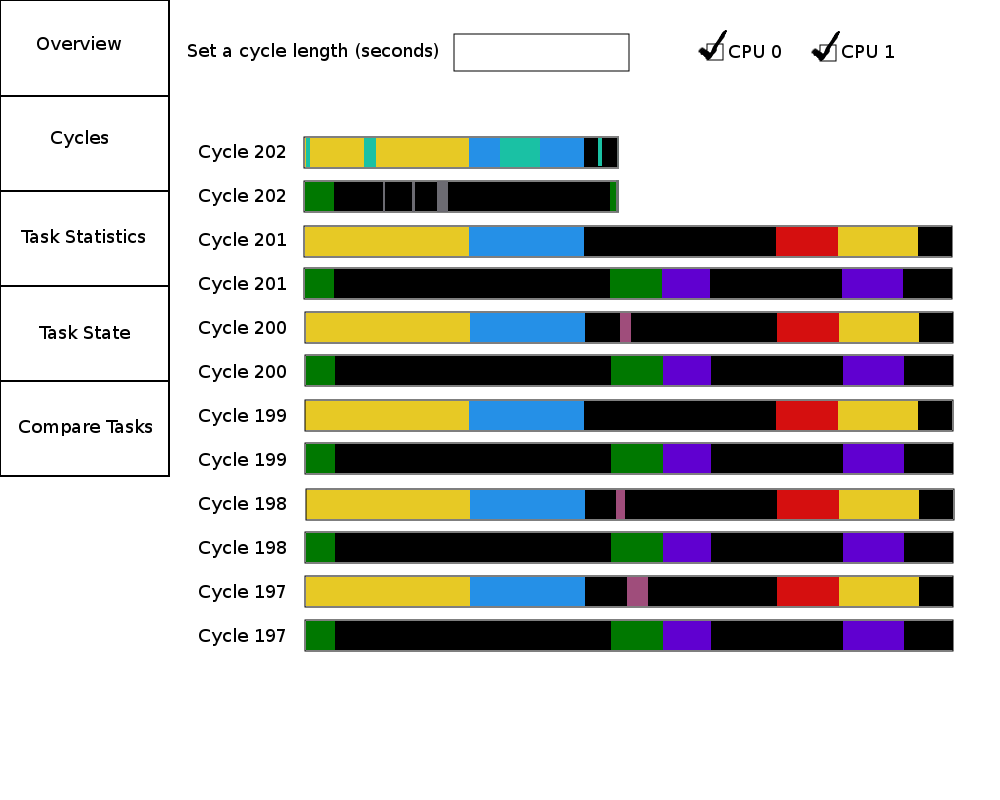
\includegraphics[width=4in]{futureCycles.png}
\caption{A mockup of how we envision the new Cycles page could look with
interleaved graphs.}
\end{center}
\end{figure}

It is also possible that the loaded files will contain more than two CPU's. For clear visual purposes, we only want to be displaying two CPU's graphs on the Cycles page. In the case that we have more than two CPU's, we would hope to be able to paginate the graphs. This does not seem to be a crucial extension of our work, since our liaisons have specifically told us that they generally expect to only have two CPU's in their trace files.


\section{Speed} %Wendy
The data SpaceX will be using with our tool is very large, and becomes even
larger once we have parsed it. As a result, some parts of the tool load slowly,
and this is something we are still working on fixing. One main fix we have
implemented is batch loading the list of events on the main page so that the
user can start interacting with the tool without waiting to load the entire
table, especially since all of the table is typically not needed.

Having done some profiling, we know that pulling data from IndexedDB is the
slowest part of our application, but at this point in time we do not have a way
to fix this.

\section{Scalability}
  Overall, the application should be made faster. We are not entirely sure how
  to improve this at the moment. IndexedDB is the slowest part of the
  application at current.

Additionally, if given files above a certain size, typically using more than 4
cores, the parsed version will be too large for IndexedDB to load, and
sometimes too large for the parser to handle as well.

There are two possibilities for fixing this. One is to prune the JSON or
finder a more compressed method of storing the data. The other is to find a
substitute for IndexedDB that is faster.


\chapter{Appendices}
\newpage
\appendix
\renewcommand{\thesection}{\Alph{section}}
\section{Example JSON} \label{App:AppendixA}

\begin{verbatim}
Tasks
{
  [name: python, pid: 34602, events: [1,5,8,23,52...], 
   preemptedBy: [kworker, systemhousekeeper,...], 
   preemptionCount: 564, totalRuntime: 10000,
   totalWaittime: 20386, totalSleeptime: 52], [name:...],

   ...   
}

Events
{
  [name: python, 
   pid: 34602, 
   cpu: 2, startTime: 12500, 
   eventType: sched_switch,
   extraInfo: prev_comm=trace-cmd prev_pid=34602 
       prev prio = 120 prev_state=S ==> next_comm=swapper/2 
       next_pid=300 next_prio=120 kworker-2418 [001]
       1681.955177, 
   activeName: kworker, 
   activePID=300], 
   [name:...], 

   ...
}
\end{verbatim}

\section{Glossary}
\begin{itemize}[ ]
\item {\bf Blocked:} When a task is runnable but another task is running on the same CPU, thereby blocking it from being able to run.
\item {\bf Cycle:} The interval between the regular deadlines that tasks running on a SpaceX rocket need to meet.
\item {\bf CPU:} The Central Processing Unit; the part of the computer that carries out instructions.
\item{\bf Event:} A specific activity of a task taking place at a single point in time that can denote a change in its state or some other action.
\item {\bf PID:} A process identifier; a number attatched to a process that is unique to that process.
\item {\bf Preemption:} When a running task is blocked by another program starting to run on the same CPU. 
\item {\bf Priority Inversion:} When a high-priority task is indirectly blocked by something of
lower priority using a shared resource that the higher priority task needs in
order to run. 
\item{\bf Process:} A program that can have many threads.
\item {\bf Running:} The state of a task when it is being executed on the CPU.
\item {\bf Task:} A single thread of a process; a series of events.
\item {\bf Waiting:} The state of a task when it cannot run, due to being blocked or waiting on some piece of information.
\end{itemize}
\end{document}




